\documentclass[hyperref={unicode},13pt,a4paper]{beamer}
\usepackage{CJKutf8}
\usepackage{bm}
\usetheme{PaloAlto}
\hypersetup{pdfpagemode={FullScreen}}

\title[并行程序设计简介]{并行程序设计简介}
\subtitle[sub]{使用Intel TBB线程库}
\author[李博群]{李博群}
\institute[SZU]{
  深圳大学,计算数学\\[1ex]
  \texttt{a14331990@163.com}
}
\date[5月 29日]{5月 29日,2014年}

\begin{document}
\begin{CJK*}{UTF8}{song}

\section{首页}
\begin{frame}[plain]
	\titlepage
\end{frame}

\section{提纲}
\begin{frame}
    \frametitle{提纲}
	\tableofcontents
\end{frame}

\section{前言}
\begin{frame}
	\frametitle{前言}
	设计并行程序的目的:
	\begin{itemize}
	\item 1. 节省时间和金钱;
	\item 2. 解决大规模或更复杂的问题;
	\item 3. 更好地利用并行硬件。
	\end{itemize}
	\begin{figure}
	\centering
	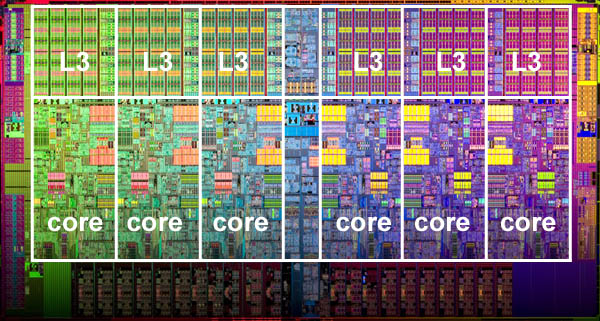
\includegraphics[width=0.8\linewidth]{intel_xeon_many_cores}
	\caption[Intel Xeon六核处理器]{Intel Xeon六核处理器} 
	\label{fig:intel_xeon_many_cores}
	\end{figure}
\end{frame}

\section{Intel TBB线程库简介}
\begin{frame}
	\frametitle{Intel TBB线程库简介}
	Intel TBB线程库(Threading Building Blocks)是由Intel开发的一个适用于多核CPU并行程序设计的C++模板库。它包含大量的适用于并行程序设计的数据结构与算法,将并行计算单元抽象为任务,将任务分配到各个CPU核心上,并动态平衡各个CPU核心上的负载。这使得程序员无需手动操作线程,简化了并行程序设计流程。
\end{frame}

\section{TBB的任务调度模型}
\begin{frame}
	\frametitle{任务调度模型}
	TBB应用任务窃取(task stealing)算法来实现多核负载平衡使得多核利用率以及性能得到提高。
	\begin{itemize}
	\item 1. 首先,所有任务被均匀分配到各个CPU核心上;
	\item 2. 当某个CPU核心完成了工作时,它将从其他仍在工作的CPU核心窃取任务。
	\end{itemize}
	\begin{figure}
	\centering
	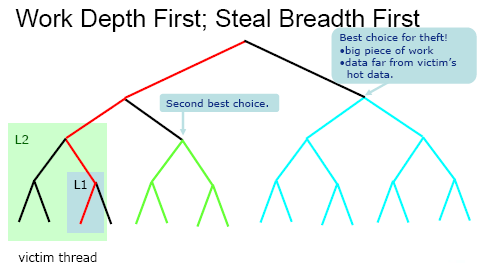
\includegraphics[width=0.7\linewidth]{tbbsteal}
	\caption[任务窃取示意图]{任务窃取示意图} 
	\label{fig:tbbsteal}
	\end{figure}	
\end{frame}

\section{TBB提供的常用并行策略}
\begin{frame}
	\frametitle{TBB提供的常用并行策略}
	TBB提供的常用并行算法框架有:
	\begin{itemize}
	\item 1. paralllel\_for,用于并行化for循环;
	\item 2. paralllel\_reduce,用于并行化分治算法。
	\end{itemize}	
\end{frame}

\begin{frame}
	\frametitle{paralllel\_for,用法与实例}
    paralllel\_for递归地将for循环的范围划分为小范围,在每个小范围上执行计算,而小范围上的计算是通过重载操作符()来实现的。
    \newline
    实例:将两个矩阵相加,代码片段-小范围的计算
	\begin{figure}
	\centering
	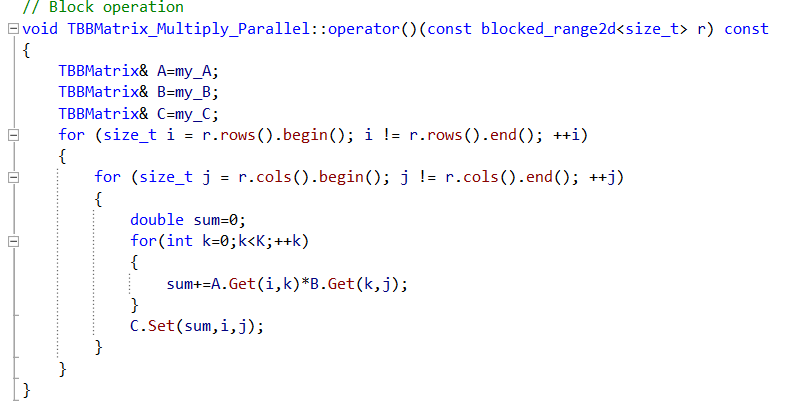
\includegraphics[width=0.87\linewidth]{parallel_for_1}
	\caption[矩阵相加代码-小范围计算]{矩阵相加代码-小范围的计算} 
	\end{figure}    
\end{frame}

\begin{frame}
	\frametitle{paralllel\_for,用法与实例-续}
    实例:将两个矩阵相加,代码片段-初始任务划分
	\begin{figure}
	\centering
	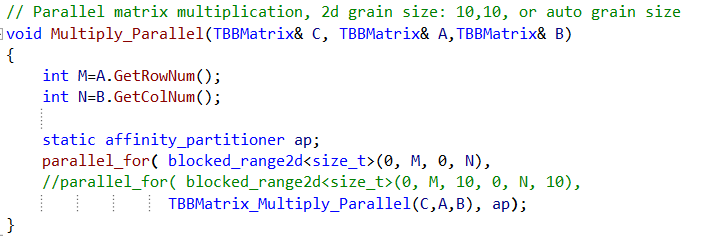
\includegraphics[width=0.87\linewidth]{parallel_for_2}
	\caption[矩阵相加代码-初始任务划分]{矩阵相加代码-初始任务划分} 
	\end{figure}    
\end{frame}

\begin{frame}
	\frametitle{paralllel\_reduce,用法与实例}
    paralllel\_reduce递归地将计算任务划分为小任务,每个小任务的计算是通过重载操作符()来实现的,最后合并所有小任务的计算结果
    \newline
    实例:将1000个数相加,代码片段-小计算任务与计算结果合并
	\begin{figure}
	\centering
	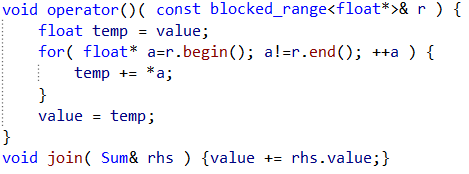
\includegraphics[width=0.87\linewidth]{parallel_reduce_1}
	\caption[1000个数相加代码-小计算任务与计算结果合并]{1000个数相加代码-小计算任务与计算结果合并} 
	\end{figure}
\end{frame}

\begin{frame}
	\frametitle{paralllel\_reduce,用法与实例-续}
    实例:将1000个数相加,代码片段-初始任务划分
	\begin{figure}
	\centering
	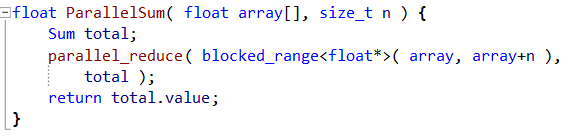
\includegraphics[width=0.87\linewidth]{parallel_reduce_2}
	\caption[1000个数相加代码-初始任务划分]{1000个数相加代码-初始任务划分} 
	\end{figure}
\end{frame}

\section{矩阵运算}
\begin{frame}
	\frametitle{TBBMatrix}
	\begin{itemize}
    \item 基于Intel TBB线程库的通用矩阵库
    \item 串行的矩阵加法和乘法
    \item 并行的矩阵加法和乘法
    \end{itemize}
\end{frame}

\begin{frame}
	\frametitle{TBBMatrix的性能测试}
    \begin{figure}
    \centering
    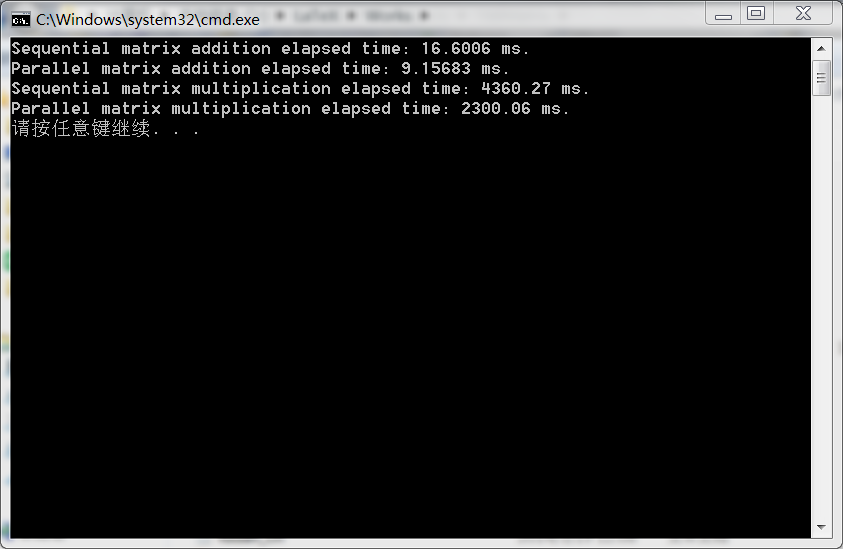
\includegraphics[width=0.9\linewidth]{tbbmatrix_performance}
    \caption[TBBMatrix的性能]{TBBMatrix的性能,测试计算机的处理器为“Intel Pentium Dual-Core E5500”} 
    \label{fig:tbbmatrix_performance}
    \end{figure}
\end{frame}

\section{格雷码解相位}
\begin{frame}
	\frametitle{TBB\_OPhase\_graycode}
	\begin{itemize}
    \item 基于Intel TBB线程库的格雷码解相位代码
    \item 串行的格雷码解相位代码
    \item 并行的格雷码解相位代码
    \end{itemize}
\end{frame}

\begin{frame}
	\frametitle{TBB\_OPhase\_graycode的性能测试}
    \begin{figure}
    \centering
    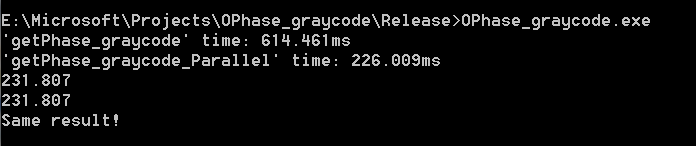
\includegraphics[width=0.9\linewidth]{tbb_ophase_graycode_performance}
    \caption[TBB\_OPhase\_graycode的性能]{TBB\_OPhase\_graycode的性能,测试计算机的处理器为“Intel Pentium Dual-Core E5500”} 
    \label{fig:tbb_ophase_graycode_performance}
    \end{figure}
\end{frame}

\section{参考文献}
\begin{frame}
	\frametitle{参考文献}
	\begin{itemize}
    \item Intel Threading Building Blocks User Guide
    \item Intel Threading Building Blocks Reference Manual
    \item The Art of Concurrency, Clay Breshears, O'Reilly, 2009
    \end{itemize}
\end{frame}

\section{思考}
\begin{frame}
	\frametitle{思考}
	并行程序设计是一项较复杂的任务,可以分解为以下几个阶段
	\begin{itemize}
    \item 1. 设计一个有合理效率的串行程序,注意这几点,模块化设计可以为以后的并行化做准备;合理效率是必要的,并行化一个效率很低的算法没有实际意义;
    \item 2. 通过分析找出关乎程序整体性能的关键模块;
    \item 3. 对关键模块采用恰当的并行策略加以并行化;
    \item 4. 调试,优化以及维护。
    \end{itemize}
\end{frame}

\section{结束}
\begin{frame}
  \begin{center}
  \emph{\Huge{谢 谢 !}}
  \end{center}
\end{frame}

\end{CJK*}
\end{document}